\chapter{Background}

\label{ch:background}

\section{Database Cracking}

Database cracking was invented by Stratos Idreos as a method of auto-tuning for database kernels by using workload-aware physical restructuring on queried columns. It forms the basis for our contributions in which we apply variants of cracking to graph algorithms with adaptive compression.

\subsection{Cracker Column}

To create an adaptive index for a relational database using a given column, we first copy that column into what is called a cracker column. When executing queries on the chosen column, we execute those queries on the cracker column using modified database operations called cracking operations. In this report we only need to use selection, however cracking can be exploited for insertion, deletion, updates and joins, as well as other operations. We will denote the cracker column by \textit{crk}.

\subsection{Cracker Select}

Initially, there is no information known about the values in the column and their locations. When a ordering query is sent to the cracker column, the column is scanned, and after the scan, all values too small to be selected appear contiguously at the start of the column, followed by all of the selected values, followed by all of the values too large to be selected. Below is an illustration indicating the effect of a cracking operation.

\begin{figure}[h]
  \centering
  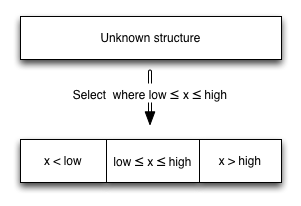
\includegraphics[]{d1_background_cracker_select}
  \caption{Cracking physically restructures the column towards being sorted}
  \label{fig:cracker_select_restructuring}
\end{figure}

Every time we perform a new cracking scan, we learn more information about the values within the column and their associated locations. Our aim is to store and exploit this information to achieve a speed up in performing queries. Notably, selections which occur first in queries are clustered first. In this way the physical layout of the cracker column is adaptive to the workload the database is under. The contiguous regions created through cracking operations are called column fragments.

\subsection{Column Fragments}

Central to the use of cracking is the concept of a column fragment. This represents a contiguous region of the cracker column whose constituent values are potentially bounded by known values. Initially, the entire column represents the only column fragment where there are no bounds yet on the values. However, as queries come in, the scans across the cracker column cause us to gain knowledge about contiguous regions of the column and the values which bound them. As we build up more knowledge about the column, the column fragments get broken up smaller and smaller, meaning that the size of our scans is decreasing as well, given that we are exploiting our knowledge about the fragments and their bounds.

The information about the column fragments is stored in the cracker index.

\subsection{Cracker Index}

The cracker index is a storage data-structure which holds the workload-aware memory about the cracker column fragments. It is denoted \textit{CrkIdx} and is subject to one invariant:

\begin{tcolorbox}
$\texttt{(value, index)}$ $\epsilon$ $\texttt{CrkIdx} \Longrightarrow \forall i < \texttt{index}: crk[i] < \texttt{value}$
\end{tcolorbox}

In plain English, if a \texttt{(value, index)} pair are stored in the cracker index, then all values before \texttt{index} in the cracker column are less than \texttt{value}.

When performing queries, we want to scan only the necessary parts of the column, so we use the information stored in the cracker index to identify the smallest column fragment which is known to contain all of the values we are looking for. After executing such a scan, we put information into the cracker index, effectively breaking up the column fragment we just scanned so that future queries will have to scan less.

\subsection{Tuple Reconstruction}

The cracker column is a copy of the original column, however, the cracking operations only apply to the cracker column, so to reconstruct original tuples based on our results from the cracker column, we use an additional array to act as the mapping between indices in the cracker column and indices in the base (original) columns. This is \textit{late} tuple reconstruction. When the cracker column is initialised, this array is also initialised, its value being an enumeration of the indices from 0 to the length of the column. We call this array the $base\_index$. All restructuring operations that happen to the cracker column also happen to the $base\_index$, in order to maintain the mapping between cracker and base columns.

\subsection{Crack-in-three Algorithm}

The algorithm we describe here as "the cracking algorithm" is actually the "crack in three" variant of the algorithm as described by Idreos. We are using this because for our use case, in which we are always selecting a single node, the crack-in-three algorithm is appropriate, whereas the simpler and faster crack-in-two scan is appropriate when querying for values one side of a given value.

The cracker select operator is called with a low value, $low$ and a high value, $high$, as well as two booleans which indicate the inclusivity of these boundaries. The select returns all the values between $low$ and $high$ in the column using the specified inclusivities.

The cracking algorithm can be grouped into five stages: Setup, tighten, scan, memo and return.

\subsubsection{Stage 1: Setup}

In the first stage of the algorithm, a contiguous section of the column is selected for scanning. If the column hasn't been cracked yet, the cracker column and $base\_index$ are initialised.

Using the arguments, we define the smallest and largest values in the selected range, which depend on the inclusivity of the range at each end.

\begin{tcolorbox}

$\sigma _{min}$ = 
\begin{math}
  \left\{
    \begin{array}{l}
      $low + 1$ \footnote{For integers, the minimum difference between elements is 1, however, for other data types, this may be different. This is discussed further in \ref{ss:perfrag}.} \texttt{, if not inclusive}\\
      $low$ \texttt{, if inclusive}
    \end{array}
  \right.
\end{math}\\
\newline{}\\
$\sigma _{max}$ = 
\begin{math}
  \left\{
    \begin{array}{l}
      $high - 1$ \texttt{, if not inclusive}\\
      $high$ \texttt{, if inclusive}
    \end{array}
  \right.
\end{math}\\
\end{tcolorbox}

We then determine the initial values for the two \textit{edge pointers}. There is a low pointer and a high pointer, which we will denote as $L$ and $H$. These two pointers are subject during the scan to the following invariants.

\begin{tcolorbox}
$(L1)$  $\forall i < L: crk[i] < \sigma _{min}$\\
$(L2)$ $crk[L] \geq \sigma _{min}$\\
$(H1)$ $\forall i > H: crk[i] > \sigma _{max}$\\
$(H2)$ $crk[H] \leq \sigma _{max}$
\end{tcolorbox}

The edge pointers then, bound the region of the cracker column in which all of the sought values lie. It would be optimal to initialise them as \textit{tightly} as possible. When we say \textit{tightly}, what we mean is as far from their associated edge as possible. For $L$ this means as close to the end of the column as possible, and for $H$ this means as close to the head of the column as possible.

To initialise the edge pointers, we search in the cracker index for values which most tightly bound the region of cracker column we have to scan. For $L$, we are looking for the value in the cracker index which is as high as possible, but no more than $low$. If no such value exists, $L$ is intialised at 0. Similarly, for $H$, we seek the value in the cracker index which is as low as possible, but no less than $high$. If no such value exists, $H$ is initialised as $|crk| - 1$.

\subsubsection{Stage 2: Tighten}

The tightening operation involves moving the two edge pointers inwards as far as possible while maintaining their invariants. In practice this is a while loop which checks the associated invariant and if it still holds, tightens the pointer (increment in the case of $L$, decrement in the case of $H$).

During this stage, it is possible to discover that no results exist. For example, if we try to select a value greater than any value in the column, then $L$ will advance all the way off the tail end. For $H$ of course, this happens when we select a value lower than any in the column, with it decrementing off the start of the column. In both of these cases, we return empty results.

Both tightening operations (low-side and high-side) are used in the next stage of the algorithm as well.

\subsubsection{Stage 3: Scan}

At the start of this stage, $L$ is duplicated to produce the \textit{iteration pointer}, denoted $I$, which is subject to a single invariant.

\begin{tcolorbox}
$\forall i: L \leq i < I, \sigma _{min} \leq crk[i] \leq \sigma _{max}$
\end{tcolorbox}

The iteration pointer is used to scan the fragment from $L$ to $H$. As $I$ encounters values within the fragment, it is determined where in the final arrangement they should lie. For example, if the value is less than $\sigma _{min}$, then it is swapped to the value at $L$, and then $L$ is tightened. This maintains the $L$ invariant, while making progress towards the situation in which only selected values are between $L$ and $H$, which is the point at which the scan in finished.

If the value at $I$ is one of the sought values, then $I$ is advanced, which maintains its invariant. Because of this, when $I$ surpasses $H$, this means that all values between $L$ and $H$ inclusive are in the selected range, and by the invariants on $L$ and $H$, every value in the selected range in the column lies between $L$ and $H$, meaning that we're finished with the scan.

Figures \ref{fig:cracking_scan_low_side_1} to \ref{fig:cracking_scan_low_side_3} show the low side swap case from the identification of the swap to the advancement of the low pointer.

\begin{figure}[H]
  \centering
  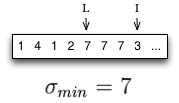
\includegraphics[]{d2_background_cracking_scan_1a}
  \caption{Standard Cracking: Low-side swap recognised}
  \label{fig:cracking_scan_low_side_1}
\end{figure}

\begin{figure}[H]
  \centering
  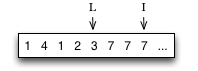
\includegraphics[]{d2_background_cracking_scan_1b}
  \caption{Standard Cracking: Low-side swap performed}
  \label{fig:cracking_scan_low_side_2}
\end{figure}

\begin{figure}[H]
  \centering
  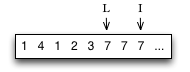
\includegraphics[]{d2_background_cracking_scan_1c}
  \caption{Standard Cracking: Low edge pointer tightened after swap}
  \label{fig:cracking_scan_low_side_3}
\end{figure}

Figures \ref{fig:cracking_scan_high_side_1} to \ref{fig:cracking_scan_high_side_3} show the same thing for the high-side swap.

\begin{figure}[H]
  \centering
  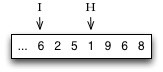
\includegraphics[]{d3_background_cracking_scan_2a}
  \caption{Standard Cracking: High-side swap recognised}
  \label{fig:cracking_scan_high_side_1}
\end{figure}


\begin{figure}[H]
  \centering
  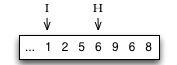
\includegraphics[]{d3_background_cracking_scan_2b}
  \caption{Standard Cracking: High-side swap performed}
  \label{fig:cracking_scan_high_side_2}
\end{figure}

\begin{figure}[H]
  \centering
  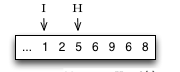
\includegraphics[]{d3_background_cracking_scan_2c}
  \caption{Standard Cracking: High edge pointer tightened after swap}
  \label{fig:cracking_scan_high_side_3}
\end{figure}

\subsubsection{Stage 4: Memo}

At this point, we know for a fact that all values before $L$ in $crk$ are also less than $\sigma _{min}$. This combination of $L$ and $\sigma _{min}$ is enough information to satisfy the main property of the cracker index, so we insert $(L, \sigma _{min})$. Additionally, we know all values before and including $H$ in $crk$ are less than $\sigma _{max}$, so all values before $H+1$ in $crk$ satisfy the required cracker index property. Hence we also insert $(H + 1, \sigma _{max})$.

\subsubsection{Stage 5: Return}

Having acquired the range of cracker column indices in which the selected values lie, we map this back to indices of the original columns using the \texttt{base\_idx} array and retrieve values from the desired column.
